% !TeX root = ../main.tex
% Add the above to each chapter to make compiling the PDF easier in some editors.
%------------------------------------------------------------------------
\chapter{Tuning Linear Programming Solvers for Query Optimization}\label{chapter:linearprogramming}

%------------------------------------------------------------------------
Our contribution consists in conducting experiments on small packing LP problems that are generated from
cardinality estimation benchmarks as mentioned in Section \ref{section:cardinality-estimate} as well as randomly generated LPs with varying sizes. We use different LP solvers, and different update methods to solve these LPs. We then proceed to compare results based on time and memory performance. We later build an analysis of our datasets' properties. Finally, we aim to give a recommendation on how to build the best performing LP solver based on the particularities of the LP problems.

%------------------------------------------------------------------------
\section{Implementation overview}
The final code repository contains 3 different solvers as shown in the
UML graph \ref{fig:hierarchy}
and a \verb|compareSolvers.cpp|, in which we can conduct our benchmarks.
\begin{figure}[htpb]
    \centering
    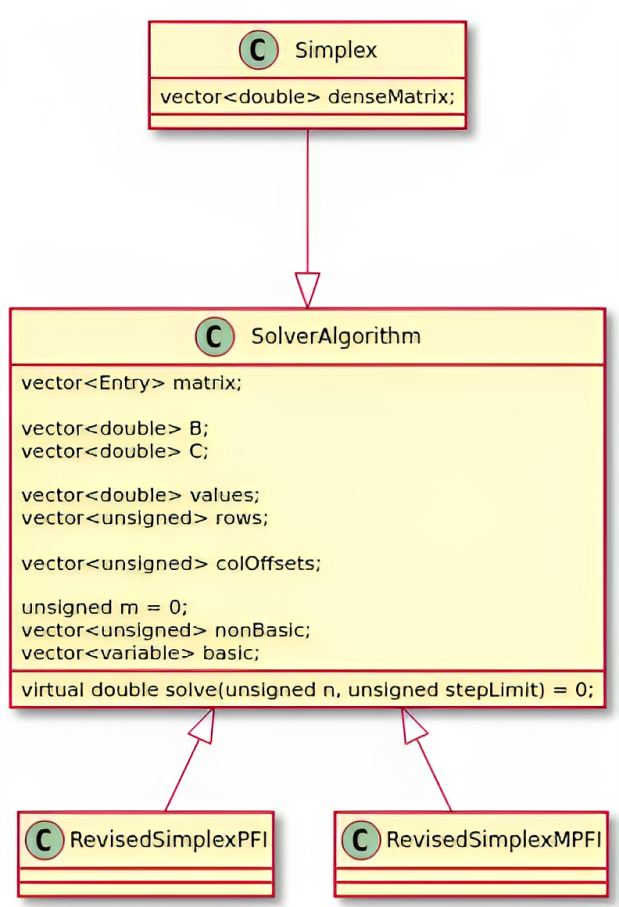
\includegraphics[height=0.6\textheight]{figures/UML.png}
    \caption{An UML Graph explaining the hierarchy of the implementation}
    \label{fig:hierarchy}
\end{figure}

%------------------------------------------------------------------------
\section{Tableau simplex solver}
This solver is the simplest of the three solvers, it follows the steps of the standard simplex
algorithm in its tabular form, see Algorithm \ref{algo:implemented_tableau}. It uses dense matrices and vectors.
Although the
texttt{doPivotting()} operation is costly (\( O(m \times n) \) where $m$ is the number of rules and
$n$ the number of variables), the simplicity of this algorithm can make it suitable for
smaller problems.
\begin{algorithm}
    \caption{Tableau Simplex Algorithm}
    \begin{algorithmic}[1]
        \State \textbf{Input:} Packing LP maximisation problem in computational form
        \State \textbf{Output:} Optimal value $z$

        \State \textbf{Step 1:} Pricing: Find pivot column, or entering variable using Bland's rule
        \State \hspace{\algorithmicindent} $enteringVars \gets \text{findPivotColumnCandidates}()$
        \State \hspace{\algorithmicindent} \textbf{if} no entering variable found \textbf{then}
        \State \hspace{\algorithmicindent} \hspace{\algorithmicindent} \text{print} "Optimal value reached."
        \State \hspace{\algorithmicindent} \hspace{\algorithmicindent} \Return $z$
        \State \hspace{\algorithmicindent} \textbf{end if}
        \State \hspace{\algorithmicindent} $pivotColumn \gets enteringVars[0]$

        \State \textbf{Step 2:} Find pivot row, or leaving variable using the ratio test
        \State \hspace{\algorithmicindent} $pivotRow \gets \text{findPivotRow}(pivotColumn)$
        \State \hspace{\algorithmicindent} \textbf{if} no leaving variable \textbf{then}
        \State \hspace{\algorithmicindent} \hspace{\algorithmicindent} \text{print} "The given LP is unbounded."
        \State \hspace{\algorithmicindent} \hspace{\algorithmicindent} \Return $\infty$
        \State \hspace{\algorithmicindent} \textbf{end if}

        \State \textbf{Step 3:} Update the tableau using pivotting and update the objective function value
        \State \hspace{\algorithmicindent} $\text{doPivotting}(pivotRow, pivotColumn, z)$

        \State \textbf{Goto Step 1}
    \end{algorithmic}
    \label{algo:implemented_tableau}
\end{algorithm}
%------------------------------------------------------------------------
\section{Data structures}

\subsection{Dense Matrix}
Given a matrix \( A \) of dimensions \( m \times n \), the density \( D \) of
the matrix is defined as:
\[
    D(A) = \frac{\text{Number of non-zero elements in } A}{m \times n}
\]
$D$ is a measure between 0 and 1, where 0 indicates a
matrix with all zero elements (completely sparse)
and 1 indicates a matrix with all non-zero elements (completely dense).

Storing a dense matrix variable \( A \) of dimensions \( m \times n \) in C++, we have two alternatives.
\begin{itemize}
    \item using a two-dimensional array. This array would contain
          $m$ arrays, representing the rows, each contains $n$ doubles, representing the matrix entries in each row.
    \item using a one-dimensional array with rows stacked next to each other.
          This array contains $m \times n$ entries.
          With the $a_{row,col}$ entry located at \texttt{A[row * (m + n) + col]}
\end{itemize}
Note that even
though there is a difference between  \texttt{array}, \texttt{vector} and \texttt{list}, we
choose \texttt{std::vector}, in all our implementation, because it suits our purpouses.
We also opt for 1D array as opposed to 2D array for better memory usage and speed.
We explain this choice:
The 2D array typically requires slightly more memory, due to the pointers in the 2D array that point to
the set of allocated 1D arrays. While this difference might seem negligible for large arrays,
it becomes relatively significant for smaller arrays.
In terms of speed, the 1D array often outperforms
the 2D array due to its contiguous memory allocation, which reduces cache misses.
While the 2D dynamic array introduces an
extra level of indirection, the 1D array has its own overhead stemming from index calculations.
However, index calculations are considered generally cheaper than indirection.
Overall, 1D vector is a better choice.

\begin{figure}[h]
    \centering
    \caption{Memory Layout of a 1D Dynamic Array}
    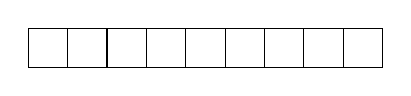
\begin{tikzpicture}[scale=0.5, every node/.style={scale=0.5}]
        \foreach \x in {0,...,8} {
                \draw (\x,0) rectangle ++(1,1);
            }
    \end{tikzpicture}
\end{figure}

\begin{figure}[h]
    \centering
    \caption{Memory Layout of a 2D Dynamic Array}
    \begin{tikzpicture}[scale=0.5, every node/.style={scale=0.5}]
        \foreach \x in {0,...,2} {
                \draw (\x,2) rectangle ++(1,1);
            }
        \foreach \x in {0,...,2} {
                \foreach \y in {0,...,2} {
                        \draw (\x*4+\y,-\x) rectangle ++(1,1);
                    }
            }
        \draw[->] (0.5,2) -- (0.5,1);
        \draw[->] (1.5,2) -- (1.5,1.25) -- (4.5,1.25) -- (4.5,0);
        \draw[->] (2.5,2) -- (2.5,1.5) -- (8.5,1.5) -- (8.5,-1);
    \end{tikzpicture}
\end{figure}


\subsection{Sparse Matrix}\label{subsubsection:sparse-matrix}
Sparsity of a matrix is a feature that can be exploited to
enhance memory complexity of our implementation, as we will discuss next.
In our dataset, we deal with sparse matrices.
We use the Compact Column Representation (CCR) format to store sparse matrices in C++. They are represented using this
structure.

\begin{verbatim}
      struct CCRMatrix {
          float *values;  // Non-zero values in the matrix
          int *rowIdx;  // Row indices corresponding to the non-zero values
          int *colPtr;  // Points to the index in `values` where each column starts
      };
\end{verbatim}

For example, consider the matrix \( A \):
\[
    A =
    \begin{bmatrix}
        5 & 0 & 0 \\
        0 & 8 & 0 \\
        0 & 0 & 3 \\
        0 & 6 & 0 \\
    \end{bmatrix}
\]

In CCR format, the matrix is represented using three arrays:
\texttt{values}, \texttt{row\_indices}, and \texttt{column\_pointers}.

\begin{align*}
    \texttt{values}           & = [5, 8, 6, 3] \\
    \texttt{row\_indices}     & = [0, 1, 3, 2] \\
    \texttt{column\_pointers} & = [0, 1, 3, 4] \\
\end{align*}


\subsection{Comparison of memory complexity}
Let's compare the memory complexity for storing a
dense matrix using a 1D vector and a sparse matrix using the Compressed Column Representation.

\textbf{Dense Matrix stored as 1D vector:}

For a matrix of size \( m \times n \):
Memory complexity: \( O(m \times n) \)

\textbf{Sparse Matrix stored with CCR format:}

Memory requirements are:
\begin{itemize}
    \item \( nnz \) for the non-zero values. Where $nnz$ is the number of non-zero values in the matrix
    \item \( nnz \) for the row indices.
    \item \( n+1 \) for column pointers.
\end{itemize}

Memory complexity: \( O(2nnz + n) \)

\textbf{Comparison:}

The best choice depends on the matrix sparsity.
If the matrix is truly dense (i.e., most of its values are non-zero), then $nnz$ approaches $m \times n$ and the dense
representation might be more appropriate. However, if the matrix is sparse, then $nnz$ is much smaller than $m \times n$
and the CCR format will be much more memory efficient.
%------------------------------------------------------------------------
\section{Revised Simplex Solver with PFI}

\begin{algorithm}
    \caption{Simplex Algorithm Using Eta Matrices}
    \begin{algorithmic}
        \State \textbf{Initialization}
        \State \textbf{Main Iteration:}
        \State \textbf{Find the Entering Variable through solving:} $yB = c_b$
        \State Initialize \(y\) to \(c_b\).
        \State Solve for \(y\) using a succession of BTRAN operations using
        eta matrices \(1\) to \(k\):
        \State Choose the first \(j\) such that \(c_j - yA_j\) is positive.
        \If{no such \(j\) exists}
        \State \Return "Optimal solution found."
        \EndIf

        \State \textbf{Find the Leaving Variable through solving:} $Bd =a$
        \State Initialize \(d\) to be the entering column $a$.
        \State Solve for \(d\) using a succession of FTRAN operations with
        eta matrices \(1\) to \(k\):
        \State Find the largest $t$ such that \( x_B^{\ast} - td \geq 0\) 
        for positive components of $d$. Choose the corresponding component as the leaving variable.
        \If{no positive entries in \(d\)}
        \State \Return "The problem is unbounded."
        \EndIf

        \State \textbf{Update the Current Basic Feasible Solution:}
        \State Set the entering variable at \(t\).
        \State Update other basic variables: \(x^*_B - td\).
        \State Push \(d\) as a new eta new eta matrix onto the vector.

        \State GOTO main iteration.
    \end{algorithmic}
\end{algorithm}
%------------------------------------------------------------------------
\section{Stability}
In numerical algorithms, small rounding errors can have a substantial impact. 
Such inaccuracies can arise from divisions by exceedingly small numbers, 
resulting in misleading outcomes.
Specifically, a zero tolerance, denoted as $\epsilon_2$, safeguards against divisions
 by extremely small numbers. These divisions tend to produce dangerous rounding errors
  and might even lead to degeneracy. An essential check in our method is to 
  ensure the diagonal entry in the eta matrix is sufficiently distant from zero; 
  otherwise, based on our experiments, the algorithm may not terminate. 

For the chosen leaving and entering variable, 
we check if the diagonal element in the eta column is smaller than $\epsilon_2$, if so,
we reject the current choice of the entering variable and proceed with the next candidate.

Typical values for computations with 15 decimal digit precision are $\epsilon_2 = 10^{-8}$
according to B.A. Murtagh \parencite{murtagh1981advanced}. 

%------------------------------------------------------------------------

